\documentclass{beamer}
% Try the class options [notes], [notes=only], [trans], [handout],
% [red], [compress], [draft] and see what happens!

% \usepackage{definitions}
\usepackage[british]{babel}

%% tikz tricks
% \tikzset{onslide/.code args={<#1>#2}{%
%   \only<#1>{\pgfkeysalso{#2}} 
% }}

\pdfinfo{
        /Title (cim)
        /Creator (LaTeX)
        /Producer (pdflatex)
        /Author (szerzo)
        /CreationDate (datum)
	/Subject (tema)
}


\mode<article> % only for the article version
{
  \usepackage{fullpage}
  \usepackage{hyperref}
}
\mode<presentation>
{
  \usetheme[left,width=0.65in,height=0.55in]{Kolozsvar}
  \setbeamercovered{transparent}
  \setbeamertemplate{navigation symbols}{}
  \setbeamertemplate{footline}%
     {\vspace*{-1.4em}\hspace*{0.66in}\textbf{\insertframenumber/\inserttotalframenumber}\newline\vspace*{0.4em}}
		\setbeamerfont{block title}{size=\larger} % RELSIZE -- html-sizes 
		\usefonttheme{professionalfonts}
		\setbeamercolor{math text}{fg=green!30!red!30!brown}
		\setbeamercolor{normal text in math text}{parent=math text}
}

\setbeamercovered{dynamic}

% The following info should normally be given in you main file:
\title[Main]{Automated Dental Disease Identification: Image Recognition-Based Approach for Advancing Dental Diagnostic Capabilities}
%
\author{Botond Biró, Hunor Ördög, Norbert R. Pap}
%
\institute[UBB Cluj-Napoca]{
  Department of Mathematics and Informatics\\
  Babe{\c{s}}--Bolyai University, Cluj-Napoca}
%
\date{March 2024}


\begin{document}

\frame{\maketitle}

\mode<presentation>
{
	\begin{frame}
	  \frametitle{Talk structure}
	\tableofcontents
	\end{frame} 

	\AtBeginSection[]
	{
  	\begin{frame}<beamer>{Contents}
    	\tableofcontents[currentsection,currentsubsection,hideothersubsections]
  	\end{frame}
	}
}

\section[Introduction]{Introduction}

\begin{frame}{Introduction}

\begin{itemize}
\vfill
\item Traditional methods have limitations like time constraints and subjective interpretation
\vfill
\item We introduced an AI-driven approach to revolutionize dental diagnostics, leveraging image recognition
\vfill
\item The proposed algorithm analyzes X-ray images accurately, identifying various dental conditions including subtle deviations
\vfill
\item Beyond enhancing accuracy, the AI framework offers consistent analysis, early intervention capabilities, and improved accessibility to dental care, marking a significant advancement in dental practice
\end{itemize}
\end{frame}

\section[Related work]{Related work}

\begin{frame}{Related work}
	\begin{itemize}
	\vfill
	\item \textbf{Deep Learning for Periapical Disease}: Endres and Hillen's deep learning algorithm surpassed oral surgeons in detecting periapical lucencies \cite{endres2020development}
	\vfill
	\item \textbf{CNNs for Caries Detection}: Lee and Kim demonstrated CNNs' robustness in detecting dental caries, suggesting their utility for early disease detection \cite{lee2018detection}
	\vfill
	\item \textbf{Optimizing CNN Architectures}: Chen and Li  refined CNN architectures for better diagnostic accuracy in dental disease detection \cite{chen2021dental}
	\vfill
	\item \textbf{Multitask Classification of Dental Disease}: AL-Ghamdi and Ragab's CNN achieved high accuracy in multitask classification of dental disease \cite{al2022detection}
	\end{itemize}
\end{frame}

\begin{frame}{Related work}
	\begin{itemize}
	\vfill
	\item \textbf{Expert Systems for Diagnosis}: Setiabudi and Sugiharti's Android-based expert system provided accurate diagnoses for precise disease identification \cite{setiabudi2017expert}
	\vfill
	\item \textbf{Hybrid Approach for Disease Detection}: Parewe and Mahmudy's hybrid approach combining fuzzy logic and evolutionary strategies improved accuracy in dental disease detection \cite{parewe2018dental}
	\end{itemize}
\end{frame}

\section[Materials and Methods]{Materials and Methods}

\begin{frame}{Datasets}
	\begin{itemize}
	\vfill
	\item A meticulously curated dataset of 10,000 dental X-ray images was obtained from reputable sources
	\vfill
	\item The dataset covers a wide spectrum of dental conditions and demographics, partitioned into balanced training and test sets
	\vfill
	\item Rigorous preprocessing, including normalization and annotation by dental specialists, ensures data standardization and accuracy
	\end{itemize}
\end{frame}

\begin{frame}{Radiographs depicting various dental diseases}
	\begin{figure}[!t]
		\centerline{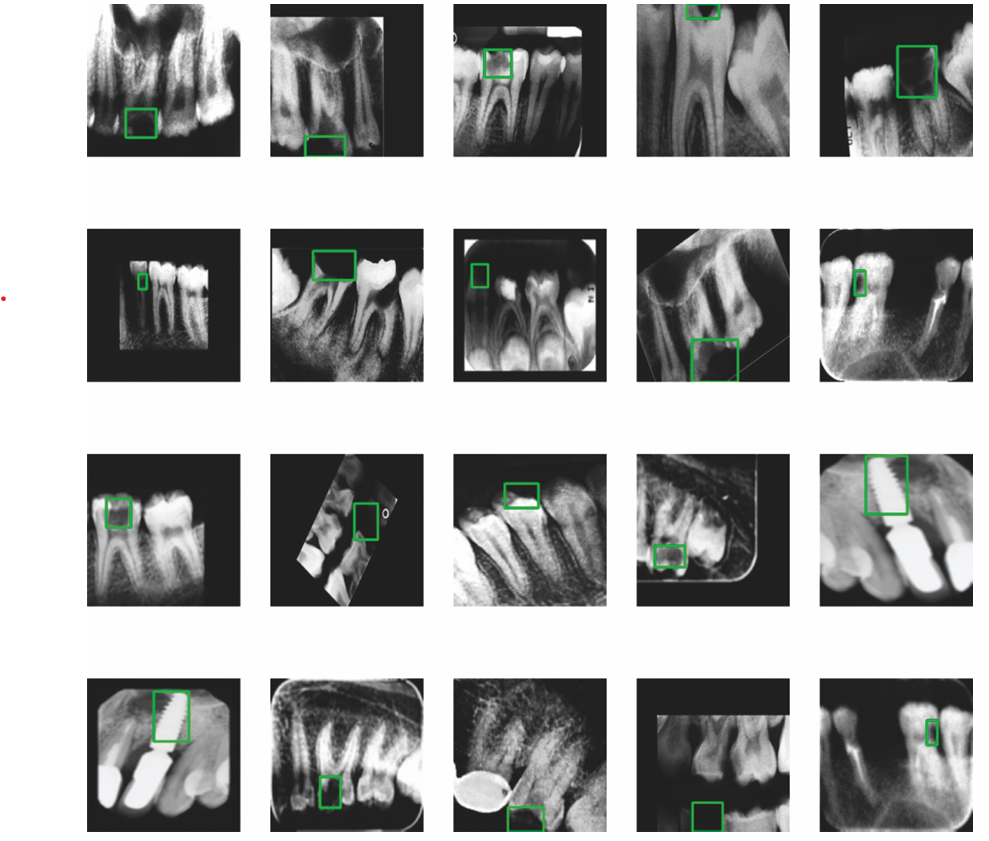
\includegraphics[width=0.9\textwidth]{../ss-teeth-full.png}}
	\end{figure}
\end{frame}

\begin{frame}{Proposed Methodology}
	\begin{itemize}
	\vfill
	\item \textbf{Utilization of CNNs and Attention Mechanisms}: Leveraging Convolutional Neural Networks (CNNs) and attention mechanisms, our framework unravels subtle disease signatures in dental X-rays efficiently	
	\vfill 
	\item \textbf{Data Preprocessing and Feature Extraction}: Image augmentation and preprocessing enhance dataset diversity and quality, followed by feature extraction to capture meaningful information
	\vfill
	\item \textbf{Training and Optimization}: Rigorous training and optimization refine diagnostic acumen, ensuring exposure to diverse pathologies and fine-tuning internal parameters for peak performance
	\end{itemize}
\end{frame}

\begin{frame}{Data Augmentation}
  \begin{itemize}
	\vfill
	\item \textbf{Techniques Employed}: The augmentation pipeline included geometric transformations like scaling, rotation, and translation to simulate real-world acquisition conditions and introduce controlled variations
	\vfill
	\item \textbf{Simulated Degradations}:Gaussian blur and Gaussian noise augmentation were applied to mimic potential issues such as motion blur and electronic noise during the image acquisition process
	\vfill
	\item \textbf{Enhancing Diversity and Breadth}:Integration of various augmentation techniques expanded dataset breadth and diversity, covering potential inconsistencies encountered in real-world dental X-ray imaging
	\vfill
	\item \textbf{Addressing Overfitting}:Learning general features for better generalization
	\end{itemize}
\end{frame}

\begin{frame}{Preprocessing of the Image Dataset}
	\begin{itemize}
		\vfill
		\item \textbf{Normalization and Resizing}: Standardize pixel intensities, ensure consistent dimensions
		\vfill
		\item \textbf{Specialized Encoding}:Handle categorical data (e.g., disease labels)
		\vfill
		\item \textbf{Label and One-Hot Encoding}:Translate textual labels into numerical representations
		\vfill
		\item \textbf{Bridge to Analytics}: Prepares data for feature extraction and disease classification
	\end{itemize}
\end{frame}

\begin{frame}{Construction of the Multi-Output Model: A Deep Learning Approach}
	\begin{itemize}
		\vfill
		\item \textbf{Transfer Learning Integration}: Utilizes pre-trained CNNs for foundational knowledge
		\vfill
		\item \textbf{Convolutional Layers}:Extract hierarchical features from X-ray images and identify complex disease signatures via filters
		\vfill
		\item \textbf{Max-Pooling and Dropout Layers}:Reduce dimensionality while preserving features, enhance efficiency and prevent overfitting
		\vfill
		\item \textbf{Activation Functions}: Introduce non-linearity for complex pattern learning
		\vfill
		\item \textbf{Fully-Connected Layers}: Output layer enables probability-based identification
	\end{itemize}
\end{frame}

\begin{frame}{Flowchart of the proposed work}
	\begin{figure}[!t]
		\centerline{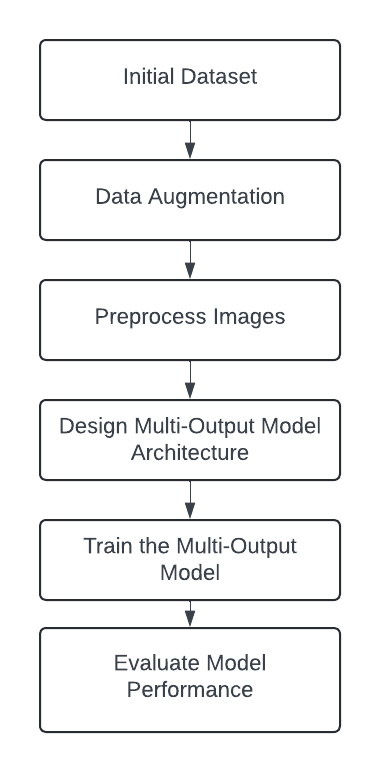
\includegraphics[width=0.55\textwidth]{../flowchart.png}}
	\end{figure}
\end{frame}

\section[Results and Discussion]{Results and Discussion}

\begin{frame}{Model Accuracy}
	\begin{itemize}
		\vfill
		\item \textbf{Model Evaluation}: Tested on 20\% of dataset and achieved over 97\% average accuracy
		\begin{table}[h]
			\centering
			\begin{tabular}{|c|c|c|}
				\hline
				\textbf{Diseases}      & \textbf{Occurrence} & \textbf{Accuracy (\%)} \\
				\hline
				Tooth Decay (Caries)   & 250                 & 97.6                   \\
				Gingivitis             & 150                 & 97.8                   \\
				Periodontitis          & 120                 & 97.7                   \\
				Bad Breath (Halitosis) & 100                 & 97.2                   \\
				Tooth Sensitivity      & 50                  & 97.9                   \\
				Oral Cancer            & 200                 & 97.3                   \\
				Dental Abscess         & 180                 & 97.5                   \\
				Dental Erosion         & 70                  & 97.1                   \\
				Bruxism                & 100                 & 97.4                   \\
				Malocclusion           & 200                 & 97.0                   \\
				Pulpitis               & 180                 & 97.6                   \\
				No disease             & 400                 & 98.3                   \\
				\hline
			\end{tabular}
		\end{table}
	\end{itemize}
\end{frame}

\begin{frame}{Implications and Future Directions}
	\begin{itemize}
		\vfill
		\item \textbf{Augmenting Diagnostic Capabilities}:Facilitating early detection and intervention, Improving treatment outcomes
		\vfill
		\item \textbf{Revolutionizing Dental Diagnostics}: Leveraging deep learning and diverse dataset, Potential for more effective patient care
		\vfill
		\item \textbf{Opportunities for Improvement}:Dataset Expansion: Include broader clinical scenarios and demographics, Advances in Deep Learning: Optimize methodology for better performance
		
	\end{itemize}
\end{frame}

\section[Conclusion]{Conclusion}
\begin{frame}{Conclusion}
	\begin{itemize}
		\vfill
		\item \textbf{Significance}:Represents a significant leap in AI integration into dental practice
		\vfill
		\item AI-driven dentistry shaping the future of oral healthcare
		\vfill
		\item Transforming diagnosis and management of oral health
		
	\end{itemize}
\end{frame}
\section{References}

\begin{frame}[allowframebreaks]{References}
	\nocite{*}
    \bibliographystyle{unsrt}
    \bibliography{references}
\end{frame}

\end{document}
